%% Run LaTeX on this file several times to get Table of Contents,
%% cross-references, and citations.

\documentclass[11pt]{book}
\usepackage{gvv-book}
\usepackage{gvv}
\usepackage[sectionbib,authoryear]{natbib}% for name-date citation comment the below line
\setcounter{secnumdepth}{3}
\setcounter{tocdepth}{2}

\makeindex

\begin{document}

\frontmatter

\booktitle{GEOMETRY}

\subtitle{Through Algebra}

\AuAff{Chakali Suresh}

\titlepage

\tableofcontents

\setcounter{page}{0}

\mainmatter

\chapter{Triangle}

Consider a triangle with vertices and midpoints      \begin{align}                                        \vec{A} = \myvec{0 \\ -5},                           \vec{B} = \myvec{-2 \\ -4},
\vec{C} = \myvec{-5 \\ -4}\\                         \vec{D} = \myvec{\frac{-7}{2} \\ -4}
\vec{E} = \myvec{\frac{-5}{2} \\ \frac{-9}{2}},
\vec{F} = \myvec{-1 \\ \frac{-9}{2}}
\end{align}

\section{Perpendicular Bisector}
\begin{enumerate}[label=\thesection.\arabic*.,ref=\thesection.\theenumi]
\numberwithin{equation}{enumi}

%Question 1.1.1:
\item The equation of the perpendicular bisector of $BC$ is
		\begin{align}
			\label{eq:tri-perp-bisect}
			\brak{\vec{x}-\frac{\vec{B}+\vec{C}}{2}}\brak{\vec{B}-\vec{C}} = 0
		\end{align}
		Substitute numerical values and find the equations of the perpendicular bisectors of $AB, BC$ and $CA$.\\
\solution\\
On substituting the values,
\begin{align}
\vec{\frac{\vec{B}+\vec{C}}{2}} &= \frac{1}{2}\myvec{-{7} \\ -8},\,
\vec{B}-\vec{C} = \myvec{3 \\ 0} 
\\
\vec{\frac{\vec{A}+\vec{B}}{2}} &= \frac{1}{2}\myvec{-2 \\ -9},\,
\vec{A}-\vec{B}=\myvec{2 \\ -1} \\
\vec{\frac{\vec{C}+\vec{A}}{2}} &= \frac{1}{2}\myvec{-5 \\ -9},\,
\vec{C}-\vec{A} = \myvec{-5 \\ 1} \\
\end{align}
yielding
\begin{alignat}{2}
  \brak{\vec{B}-\vec{C}}^{\top}\brak{\frac{\vec{B}+\vec{C}}{2}} 
	&= \myvec{3 & 0}\myvec{\frac{7}{2} \\ -4}
	&&= \frac{-21}{2}
  \\
\brak{\vec{A}-\vec{B}}^{\top}\brak{\frac{\vec{A}+\vec{B}}{2}}
	&= \myvec{2 & -1}\myvec{-1 \\ \frac{-9}{2}}
	&&= \frac{5}{2}
  \\
\brak{\vec{C}-\vec{A}}^{\top}\brak{\frac{\vec{C}+\vec{A}}{2}}
	&= \myvec{-5 & 1}\myvec{\frac{-5}{2} \\ \frac{-9}{2}}
	&&= 8
\end{alignat}
Thus, the perpendicular bisectors are obtained from as
		\begin{alignat}{2}
			BC&: \quad \myvec{3 & 0}\vec{x} &&= \frac{-21}{2}\\
			CA&: \quad \myvec{2 & -1}\vec{x} &&= \frac{5}{2}\\
			AB&: \quad \myvec{-5 & 1}\vec{x} &&= 8
		\end{alignat}
		\begin{figure}[H]
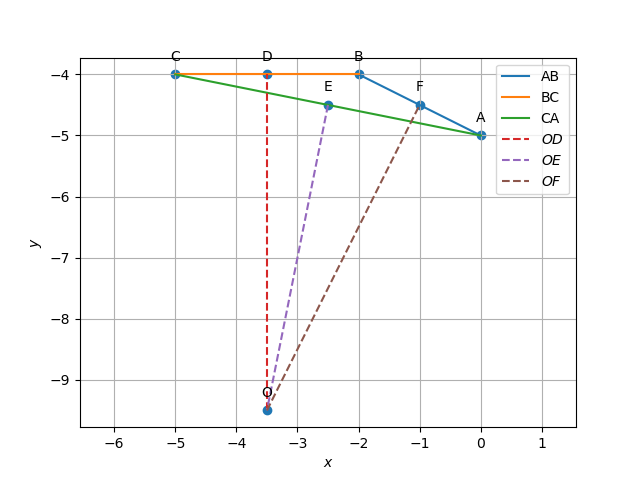
\includegraphics[width=\columnwidth]{/sdcard/Documents/figs/perp_bisect}
\caption{Perpendicular Bisectors of $\triangle ABC$}
\label{fig:Perpendicular bisectors }
\end{figure}

%Question 1.1.2:
\item Find the intersection $\vec{O}$ of the perpendicular bisectors of $AB$ and $AC$.\\
\solution\\
Given vector equation of perpendicular bisector of $\vec{A}-\vec{B}$ is
\begin{align}
 (\vec{A}-\vec{B})^\top  \brak{ \vec{x} - \frac{\vec{A}+\vec{B}}{2}} = 0
\end{align}
where,
\begin{align}
\vec{A}+\vec{B} &= \myvec{-2 \\-9}\\
\vec{A}-\vec{B} &= \myvec{2 \\ -1}\\
\implies (\vec{A}-\vec{B})^\top &= \myvec{2 & -1}
\end{align}
$\therefore $ The vector equation of $\vec{O}-\vec{F}$ is
\begin{align}
\myvec{2 & -1} \brak{ \vec{x}-\frac{1}{2}\myvec{-2 \\ -9} } &= 0\\
\implies \myvec{2 & -1}\vec{x} &= \frac{1}{2}\myvec{2 & -1}\myvec{-2 \\ -9}\\
\myvec{2 & -1}\vec{x} &= \frac{5}{2}
\end{align}\\
Vector equation of perpendicular bisector of $\vec{A}-\vec{C}$ is
\begin{align}
(\vec{A}-\vec{C})^\top\brak{ \vec{x} - \frac{\vec{A}+\vec{C}}{2}} = 0
\end{align}
where,
\begin{align}
\vec{A}+\vec{C} &= \myvec{-5 \\ -9}\\
\vec{A}-\vec{C} &= \myvec{5 \\ -1}\\
\implies (\vec{A}-\vec{C})^\top &= \myvec{5 & -1}
\end{align}
$\therefore $ The vector equatio of $\vec{O}-\vec{E}$ is
\begin{align}
\myvec{5 & -1}\brak{ \vec{x}-\frac{1}{2}\myvec{-5\\-9}} &= 0\\
\implies \myvec{5 & -1}\vec{x} &= \frac{1}{2}\myvec{5 & -1}\myvec{-5\\-9}\\
\myvec{5 & -1}\vec{x} &= -8
\end{align}
Thus,
\begin{align}
\myvec{2 & -1& \frac{5}{2} \\ 5 & -1 & -8} &\xleftrightarrow[]{R_1 \leftarrow \frac{R1}{2}} \myvec{1 & \frac{-1}{2} & \frac{-5}{4} \\ 5 & 1 & -8}\\
&\xleftrightarrow[]{R_2 \leftarrow R2-5R1}
\myvec{1 & \frac{-1}{2} & \frac{-5}{4} \\ 0 & \frac{3}{2} & \frac{-57}{4}}\\ 
&\xleftrightarrow[]{R_2\leftarrow \frac{2R_2}{3}} \myvec{1 & \frac{-1}{2} & \frac{-5}{4} \\ 0 & 1 & \frac{-19}{2}}\\
&\xleftrightarrow[]{R_1\leftarrow R_1 + \frac{R_2}{2}}
 \myvec{1 & 0 & \frac{-7}{2} \\ 0 & 1 & \frac{-19}{2}}
\end{align}
Therefore, the point of intersection of perpendicular bisectors of $\vec{A}-\vec{B}$ and $\vec{A}-\vec{C}$ is $\vec{O} = \frac{1}{2}\myvec{-7 \\ -19}$
		\begin{figure}[H]
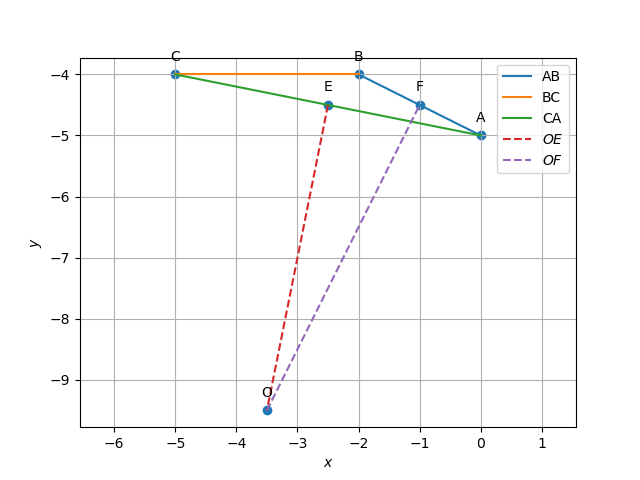
\includegraphics[width=\columnwidth]{/sdcard/Documents/figs/perp_bisect2}
			\caption{Perpendicular Bisectors $\vec{OE,OF }$of $\vec{AC,AB}$}
\label{fig:Bisectors OE,OF}
\end{figure}

%Question 1.1.3:
\item Verify that $\vec{O}$ satisfies
			\eqref{eq:tri-perp-bisect}.
$\vec{O}$ is known as the circumcentre.\\
\solution\\
 From the previous question we get,
 \begin{align}
	\vec{O}&=\frac{1}{2} \myvec{-7 \\ -19}
\end{align}
when substituted in the above equation,
\begin{align}
	&= \brak{\vec{O}-\frac{\vec{B}+\vec{C}}{2}}.\brak{\vec{B}-\vec{C}}\\
	&= \brak{\frac{1}{2}\myvec{-7 \\ -19}- \frac{1}{2}\myvec{-7 \\ -8}}^{\top} \myvec{3 \\ 0}\\
	&= \frac{1}{2}\myvec{0 & -11}\myvec{3 \\ 0}\\
	&= 0
\end{align}
It is hence proved that $\vec{O}$ satisfies the equation \eqref{eq:tri-perp-bisect}
\begin{figure}[H]                                         
	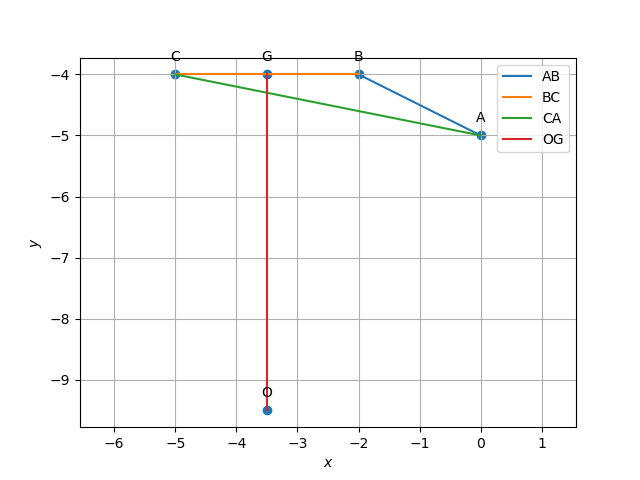
\includegraphics[width=\columnwidth]{/sdcard/Documents/figs/circumcenter}
	\caption{Circumcenter($\vec{OG}$) of $\triangle ABC$}
\label{fig:circumcenter OG}      
\end{figure}

%Question 1.1.4:
\item Verify that 
		\begin{align}
			OA = OB = OC 
		\end{align}
  \solution\\
Given,
\begin{align}
    \vec{O - A} &= \frac{1}{2}\myvec{-7 \\ -19} - \myvec{0 \\ -5}\\
    &= \myvec{\frac{-7}{2} \\ \frac{-9}{2}}\\
    \vec{O - B} &= \frac{1}{2}\myvec{-7 \\ -19} - \myvec{-2 \\ -4}\\
    &= \myvec{\frac{-3}{2} \\ \frac{-11}{2}}\\
    \vec{O - A} &= \frac{1}{2}\myvec{-7 \\ -19} - \myvec{-5 \\ -4}\\
    &= \myvec{\frac{3}{2} \\ \frac{-11}{2}}
\end{align}
By substituting the above values
\begin{enumerate}
\item 
\begin{align}
\vec{OA} &= \sqrt{(\vec{O}-\vec{A})^{\top}(\vec{O}-\vec{A})}\\
&= \sqrt{\myvec{\frac{-7}{2} & \frac{-9}{2}} \myvec{\frac{-7}{2} \\ \frac{-9}{2}}}\\
 &= \sqrt{\frac{-7}{2}^2 + \frac{-9}{2}^2}\\
 &= \frac{\sqrt{130}}{2}
\end{align}
\item 
\begin{align}
\vec{OB} &= \sqrt{(\vec{O}-\vec{B})^{\top}(\vec{O}-\vec{B})}\\
 &= \sqrt{\myvec{\frac{-3}{2} & \frac{-11}{2}} \myvec{\frac{-3}{2} \\ \frac{-11}{2}}}\\
 &= \sqrt{\frac{-3}{2}^2 + \frac{-11}{2}^2}\\
 &= \frac{\sqrt{130}}{2}
\end{align}
\item 
\begin{align}
OC &= \sqrt{(\vec{O}-\vec{C})^{\top}(\vec{O}-\vec{C})}\\
 &= \sqrt{\myvec{\frac{3}{2} & \frac{-11}{2}}  \myvec{\frac{3}{2} \\ \frac{-11}{2}}}\\
&= \sqrt{\frac{3}{2}^2 + \frac{-11}{2}^2}\\
 &= \frac{\sqrt{130}}{2}
\end{align}
\end{enumerate}
From above, 
\begin{align}
\vec{OA = OB = OC}
\end{align}

%Question 1.1.5:
	\item Draw the circle with centre at $\vec{O}$ and radius 
		\begin{align}
			\vec{R = OA}
		\end{align}
		This is known as the {\em circumradius}. \\
  \solution\\
  \begin{align}
\vec{O} = \frac{1}{2}\myvec{-7 \\ -19}
\end{align}
Now we will calculate the radius,
\begin{align}
      R &= OA\\
        &= \norm{\vec{A} - \vec{O}}\\
        &= \norm{\myvec{0 \\ -5} - \frac{1}{2}\myvec{-7 \\ -19}}\\
        &= \norm{\myvec{\frac{7}{2} \\ \frac{9}{2}}}\\
        &= \frac{\sqrt{130}}{2}
\end{align}
\begin{figure}[H]                                                                                                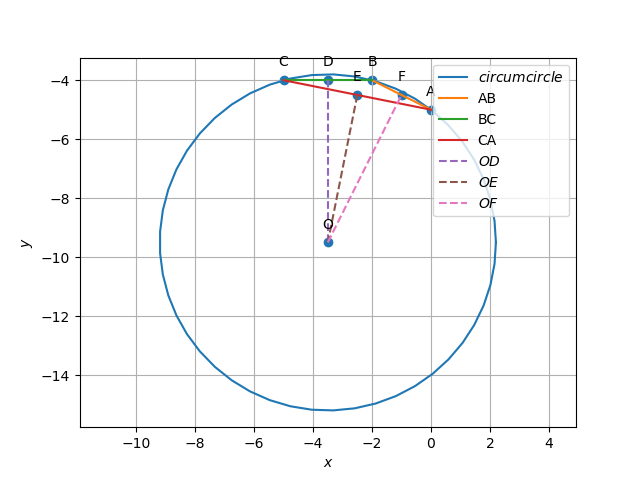
\includegraphics[width=\columnwidth]{/sdcard/Documents/figs/circumcircle}
        \caption{Circumcircle of $\triangle ABC$ with center $\vec{O}$}
\label{fig:circumcircle}
\end{figure}

%Question 1.1.6:
\item Verify that 
		\begin{align}
			\angle BOC = 2\angle BAC.
		\end{align}\\
\solution\\
We have a point $\vec{O}=\myvec{\frac{-7}{2}\\\frac{-19}{2}}$
which is intersection point of the perpendicular bisectors of AB and AC and is circumcentre of the triangle made by points A,B and C.

\begin{enumerate}
\item To find  the value of $\angle{BOC}$ :
\begin{align}
\vec{B}-\vec{O}
          &= \myvec{\frac{3}{2}\\\frac{11}{2}}\\
\vec{C}-\vec{O}
          &= \myvec{\frac{-3}{2}\\\frac{11}{2}}
\end{align}
calculating the norm of $\vec{B}-\vec{O}$ and $\vec{C}-\vec{O}$,we get:
\begin{align}
	\norm{\vec{B}-\vec{O}} &= \frac{\sqrt{130}}{2}\\
	\norm{\vec{C}-\vec{O}} &= \frac{\sqrt{130}}{2}
\end{align}
by doing matrix multiplication, we get:
\begin{align}
\brak{\vec{B}-\vec{O}}^{\top}\brak{\vec{C}-\vec{O}} &= 28
\end{align}
to calcuate the $\angle{BOC}$:
\begin{align}
\cos{BOC} &= \frac{\brak{\vec{B}-\vec{O}}^{\top}\brak{\vec{C}-\vec{O}}}{\norm{\vec{B}-\vec{O}}\norm{\vec{C}-\vec{O}}}\\
&= \frac{28}{\frac{\sqrt{130}}{2}\times\frac{\sqrt{130}}{2}}\\
&= \frac{112}{130}\\
\implies\angle{BOC}&=\cos^{-1}\brak{\frac{112}{130}}\\
	&= 30.5\degree
\end{align}
Taking the reflex of above angle we get
		\begin{align}
			\angle{BOC} &= 360\degree - 30.5\degree
			&= 329.5\degree\label{eq:1}
		\end{align}

	\item To find  the value of $\angle{BAC}$ :
\begin{align}
\vec{B}-\vec{A} &= \myvec{-2\\1}\\
\vec{C}-\vec{A} &= \myvec{5\\-1}
\end{align}
calculating the norm of $\vec{B}-\vec{A}$ and $\vec{C}-\vec{A}$,we get:
\begin{align}
	\norm{\vec{B}-\vec{A}} &= \sqrt{5}\\
	\norm{\vec{C}-\vec{A}} &= \sqrt{26}
\end{align}
by doing matrix multiplication, we get:
\begin{align}
\brak{\vec{B}-\vec{A}}^{\top}\brak{\vec{C}-\vec{A}} &= -11
\end{align}
to calcuate the $\angle{BAC}$:
\begin{align}
\cos{BAC} &= \frac{\brak{\vec{B}-\vec{A}}^{\top}\brak{\vec{C}-\vec{A}}}{\norm{\vec{B}-\vec{A}}\norm{\vec{C}-\vec{A}}}\\
&= \frac{-11}{\sqrt{5}\times\sqrt{26}}\\
&= \frac{-11}{\sqrt{130}}\\
	\implies\angle{BAC} &= \cos^{-1}\brak{\frac{-11}{\sqrt{130}}}\\
&= 164.75\degree \label{eq:2}
\end{align}
from equation \eqref{eq:2}: 
\begin{align}
2\times\angle{BAC} = 329.5\degree \label{eq:3}
\end{align}
On comparing equation \eqref{eq:1} and equation \eqref{eq:3}:
\begin{align}
\angle{BOC} = 2\times\angle{BAC}
\end{align}
Hence,verified.
\end{enumerate}

%Question 1.1.7
\item Let 
\begin{align}
\vec{P} = \myvec{\cos \theta & -\sin \theta \\ \sin \theta & \cos \theta}
\end{align}
Find $\theta$ if 
\begin{align}
\vec{C}-\vec{O}=\vec{P}\brak{\vec{A}-\vec{O}}
\end{align}
\solution
\begin{align}
    \vec{C}-\vec{O}
	  & =\myvec{\frac{-3}{2}\\\frac{11}{2}}\\
\vec{A}-\vec{O}
	 & =\myvec{\frac{7}{2}\\\frac{9}{2}}
	  \\
\vec{P} &= \myvec{\cos \theta & -\sin \theta \\ \sin \theta & \cos \theta} \\
   \vec{C}-\vec{O}&=\vec{P}\brak{\vec{A}-\vec{O}} \label{eq:1.4.7.6}
\end{align}
 Now from \eqref{eq:1.4.7.6}
 \begin{align}
 \myvec{\frac{-3}{2}\\\frac{11}{2}} &= \myvec{\cos \theta & -\sin \theta \\ \sin \theta & \cos \theta} \myvec{\frac{7}{2}\\\frac{9}{2}}    
 \end{align}
solving using matrix multiplication,we get
\begin{align}
	\myvec{\frac{-3}{2}\\\frac{11}{2}} &= \myvec{ \frac{7}{2}\cos\theta - \frac{9}{2}\sin\theta \\ \frac{7}{2}\sin\theta + \frac{9}{2}\cos\theta}
\end{align}
Comparing on Both sides ,we get
\begin{align}
     7\cos\theta - 9\sin\theta &= -3   \label{eq:1.4.7.9}\\
 7\sin\theta + 9\cos\theta &= 11 \label{eq:1.4.7.10}
\end{align}
On solving equations \eqref{eq:1.4.7.9}  and \eqref{eq:1.4.7.10}
\begin{align}
    \cos\theta&= \frac{3}{5} \\
    \sin\theta&= \frac{4}{5} \\
    \theta &=\cos^{-1}\frac{3}{5} \\
            &= 53.13 \\
	    \therefore \theta &= 53.13
\end{align}
\end{enumerate}

\latexprintindex
\end{document}
